\documentclass[doc, 12pt, a4paper, draftall]{apa7th-TESIS-USIL} % Document class

\usepackage{lipsum} % Generar texto ficticio Lorem Ipsum
\usepackage[american]{babel} % Configuración del idioma en español
\usepackage[utf8]{inputenc}
\usepackage[T1]{fontenc}
\usepackage{csquotes} % Mejora las citas y referencias bibliográficas
\usepackage[backend=biber, style=apa]{biblatex} % Estilo APA para citas y referencias bibliográficas
\addbibresource{20_Bibliography/bibliography.bib} 
\usepackage{hyperref} % Creación de enlaces internos y externos en el documento PDF
\hypersetup{
    colorlinks=true, % Activar enlaces coloreados
    linkcolor=black, % Color de los enlaces internos (por defecto: red)
    citecolor=black, % Color de los enlaces de citas (por defecto: green)
    urlcolor=black, % Color de los enlaces URL (por defecto: magenta)
    linkbordercolor=white, % Color del borde de los enlaces internos (por defecto: red)
    citebordercolor=white, % Color del borde de los enlaces de citas (por defecto: green)
    urlbordercolor=white % Color del borde de los enlaces URL (por defecto: magenta)
}
\usepackage{subcaption} % Permite crear subfiguras
\usepackage{mathptmx} % Cargar la fuente Times New Roman

%%%%%%%%% INCLUIR Y NUMERAR SECCIONES EN TOC Y DOCUMENTO %%%%%%%%%%%%%

\setcounter{tocdepth}{2} % Incluir hasta nivel de subsecciones en la tabla de contenidos
\setcounter{secnumdepth}{3} % Numerar hasta nivel de subsecciones
\AtBeginDocument{\addtocontents{toc}{\protect\thispagestyle{empty}}} % Desactivar numeración de página en la página de la tabla de contenidos

%%%%%%%%% AGREGAR PREFIJO A LOF Y LOT %%%%%%%%%%%%%

\renewcommand{\cftfigpresnum}{Figura }
\setlength{\cftfignumwidth}{5em}

\renewcommand{\cfttabpresnum}{Tabla }
\setlength{\cfttabnumwidth}{5em}

\renewcommand{\cftmyequationspresnum}{Ecuación }
\setlength{\cftmyequationsnumwidth}{6em}

%%%%%%%%% MODIFICAR ENTORNO SUBFIGURE %%%%%%%%%%%%%

\renewcommand\thesubfigure{\Alph{subfigure}}
\captionsetup[subfigure]{labelformat=empty}

%%%%%%%%%% Centrado del título del ÍNDICE / LISTA DE FIGURAS / LISTA DE CUADROS %%%%%%%%%

\renewcommand{\cfttoctitlefont}{\hfill \normalfont\normalsize\bfseries}
\renewcommand{\cftaftertoctitle}{\hfill}

\renewcommand{\cftlottitlefont}{\hfill\normalfont\normalsize\bfseries}
\renewcommand{\cftafterlottitle}{\hfill}

\renewcommand{\cftloftitlefont}{\hfill\normalfont\normalsize\bfseries}
\renewcommand{\cftafterloftitle}{\hfill}

\renewcommand{\listequationsname}{\hfill\normalfont\normalsize\bfseries Lista de Ecuaciones \hfill}

\renewcommand{\listofabbreviationsname}{\hfill\normalfont\normalsize\bfseries Lista de Siglas \hfill}

\renewcommand{\listofsymbolsname}{\hfill\normalfont\normalsize\bfseries Lista de Simbolos \hfill}

%%%%%%%%%% AGREGAR PREFIJO DE A SECCIONES Y A TOC %%%%%%%%%

\makeatletter
% Agregar prefijo a las secciones en la tabla de contenidos
%\renewcommand{\cftsecpresnum}{Capítulo }
%\renewcommand{\cftsecaftersnum}{:}
\settowidth{\cftsecnumwidth}{\normalfont\bfseries\thesection\hspace{1em}} % Calcula el ancho necesario
\addtolength{\cftsecnumwidth}{1.0em} % Agrega un espaciado adicional
\makeatother

\setlength{\cftbeforesecskip}{2mm}
\renewcommand\cftsecafterpnum{\vskip5pt}
\renewcommand\cftsubsecafterpnum{\vskip5pt}
\renewcommand\cftsubsubsecafterpnum{\vskip5pt}

%%%%%%%%%%%%%% DEFINIR INFORMACIÓN PERSONAL Y TRABAJO %%%%%%%%%%%%%%%%%%%%

%Título de la DOCUMENTO (Siempre en mayuscula y sin saltos de linea)
\title{PROPUESTA DE IMPLEMENTACIÓN DE UN REFORZAMIENTO ESTRUCTURAL PARA REDUCIR LA VULNERABILIDAD SÍSMICA DE LA IGLESIA VILLA DE HUAYLLAY USANDO MODELO DE ELEMENTOS FINITOS}

%Título corto del DOCUMENTO al pie de PÁGINA (Agregar salto de línea de ser necesario)
\shorttitle{PROPUESTA DE IMPLEMENTACIÓN DE UN REFORZAMIENTO ESTRUCTURAL PARA REDUCIR LA VULNERABILIDAD SÍSMICA DE LA IGLESIA VILLA DE HUAYLLAY USANDO MODELO DE ELEMENTOS FINITOS}

%Nombre de la FACULTAD (Siempre en mayuscula)
\faculty{FACULTAD DE INGENIERÍA}

%Para obtener el GRADO profesional de ...
\degree{Ingeniería Civil}

%AUTOR para carátula (Siempre en mayuscula y sin saltos de linea)
\authorname{SANCHEZ CARBAJAL, DINER ERICK}
\authororcid{(XXXX-XXXX-XXXX-XXXX)}

%ASESOR para carátula (Siempre en mayuscula y sin saltos de linea)
\advisorname{ING. SOTO OBLEA, EDWARD JONATHAN}
\advisororcid{(XXXX-XXXX-XXXX-0000)}

%AÑO para carátula
\yyearr{2023}
 % Call preamble using input

\begin{document}

% Carátula del documento
% Titlepage:
\maketitle

% Epígrafe
\begin{epigraph}
    \hfill {\fontsize{9}{13}\selectfont \hfill A mis queridos padres Edgar y Alberta, por  su apoyo, comprensión y concejos. A mis hermanos por alegrarme en los momentos más importantes de mi vida. A mis queridos padres Edgar y Alberta,  por  su apoyo concejos. A mis hermanos por alegrarme en los momentos más importa mi vida.} 
\end{epigraph}

\frontmatter % Comenzar numeración romana

% Índice de contenidos
\renewcommand\contentsname{\centering Índice}
\tableofcontents
\newpage
% Índice de tablas
\renewcommand\listtablename{\centering Índice de Tablas}
\listoftables
\newpage
% Índice de figuras
\renewcommand\listfigurename{\centering Índice de Figuras}
\listoffigures
\newpage
\doublespacing

% Dedicatoria
\begin{dedication}
    \hfill {\fontsize{8}{13}\selectfont A mis queridos padres Edgar y Alberta,  por  su apoyo, comprensión  y  concejos. A mis hermanos por alegrarme en los momentos más importantes de mi vida.}
\end{dedication}  

% Agradecimientos
\begin{acknowledgments}
    Acknowledgments here! \lipsum[41]
\end{acknowledgments}

% Resumen
\begin{resumen}
    Resumen aquí
\end{resumen}

% Abstract
\begin{abstract}
    Abstract here
\end{abstract}

\mainmatter % Comenzar numeración arábica

% Capítulo I: Introducción
% Chapter I:
\section{Introducción}

\lipsum[2]

\lipsum[3]

\lipsum[4]

% Capítulo II: Planteamiento del Problema
% Chapter II:
\section{Planteamiento del Problema}

  % Section 2.1:
\subsection{Situación Problemática}

\Textcite{vonDavier2011} said this, that
too \parencite{vonDavier2011,Lassen2006}.  Further evidence comes from
other sources \parencite{Shotton1989,Lassen2006}.


  % Section 2.2:
\subsection{Formulación del Problema}

\lipsum[5]

\begin{figure}[ht]
  \caption[Cuadro y gráficos que muestran el método N2]{Cuadro y gráficos que muestran el método N2. Adaptado de \cite{Gilbert2004}}
  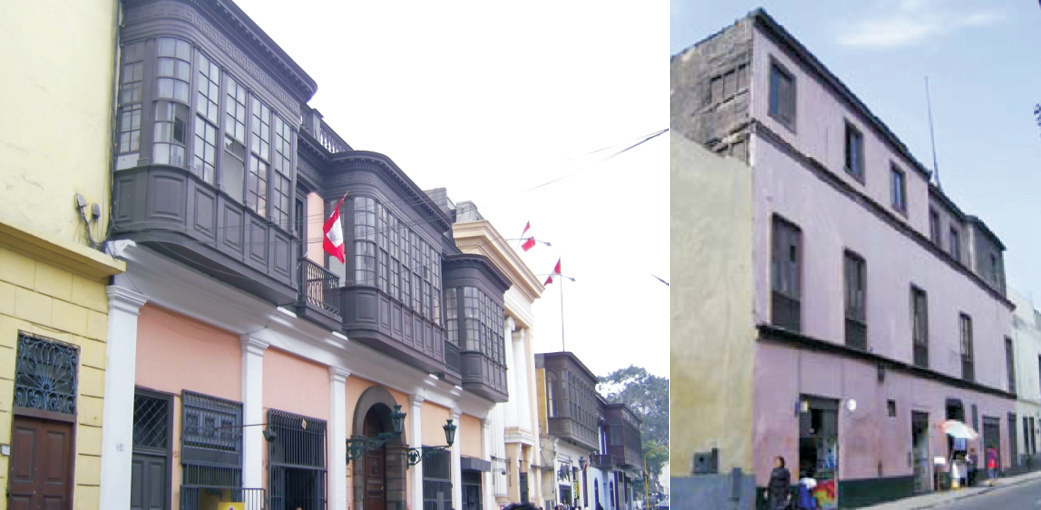
\includegraphics[scale=0.36]{F_Figures/12_Chapter III/Cap3_Imagen20.png}
  \figurenote{This is a great figure.}
	\label{Cap3_Figura8}
\end{figure}

  % Section 1.3:
\subsection{Justificación de la Investigación}

\lipsum[6]

  % Section 2.4:
\subsection{Objetivos de la Investigación}

\lipsum[7]

\subsubsection{Objetivo General}

\lipsum[8]

\subsubsection{Objetivos Específicos}

\lipsum[10]

\begin{figure}[ht]
  \caption{Figura con subfiguras}
  \label{fig:figura}
  \begin{subfigure}{0.35\textwidth}
      \centering
      \caption{A}
      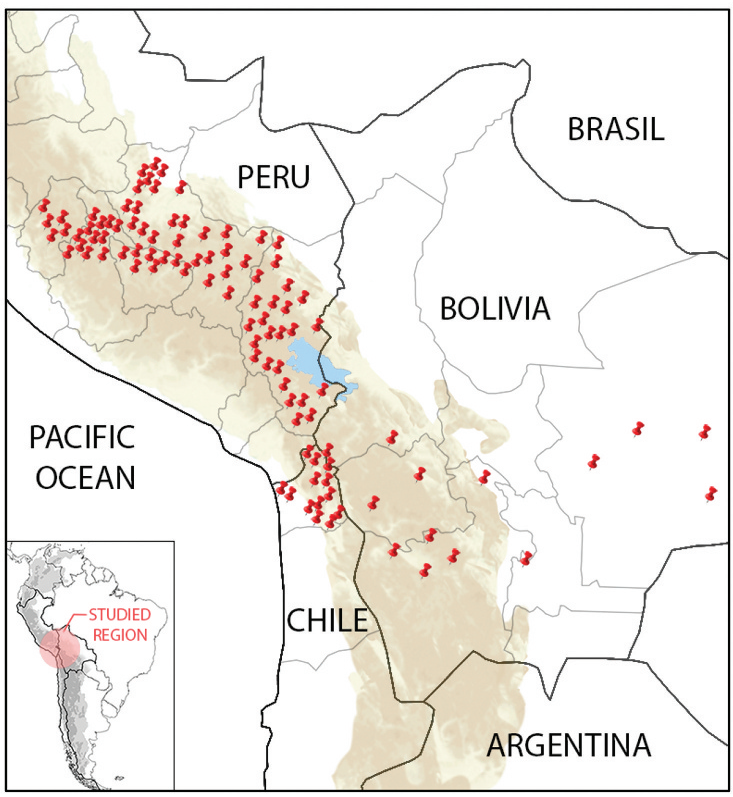
\includegraphics[scale=0.28]{F_Figures/11_Chapter II/Cap2_Imagen2a.png}
      \label{fig:subfig1}
  \end{subfigure}
  \hfill
  \begin{subfigure}{0.55\textwidth}
      \centering
      \caption{B}
      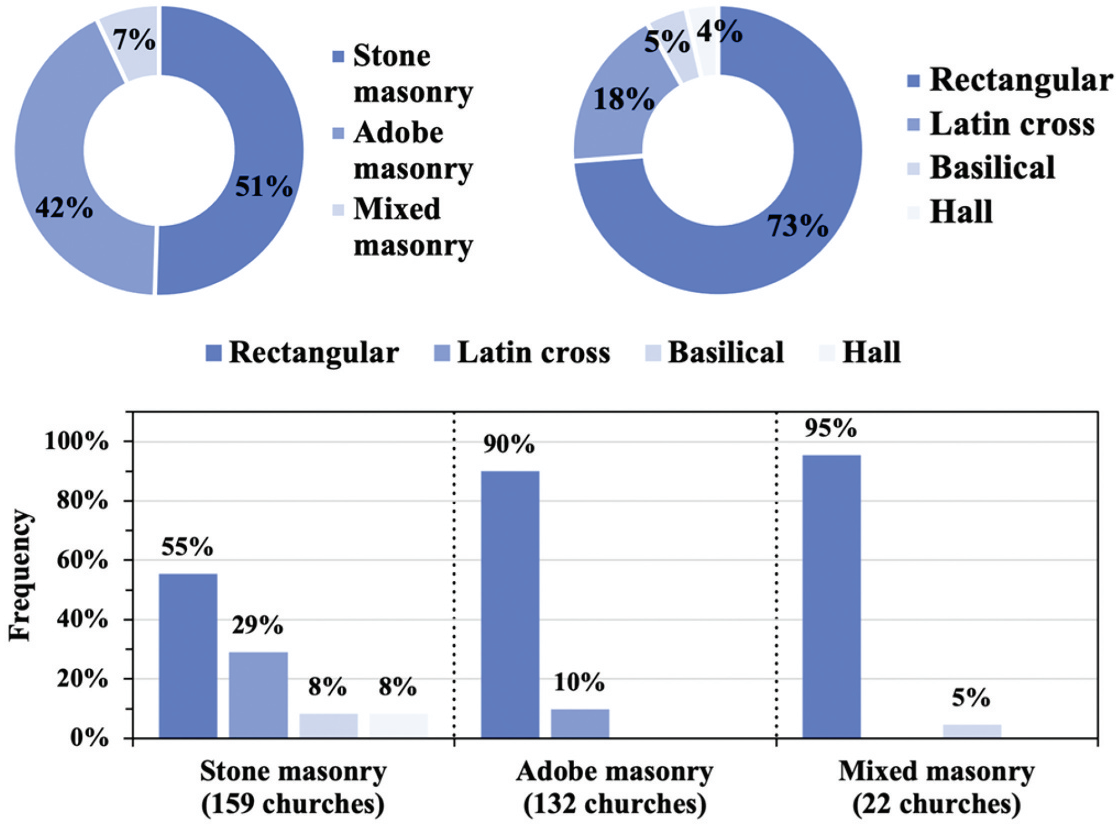
\includegraphics[scale=0.28]{F_Figures/11_Chapter II/Cap2_Imagen2b.png}
      \label{fig:subfig2}
  \end{subfigure}
  \figurenote{Buenas figuras}
\end{figure}

\subparagraph{Inter-rater reliability}
\lipsum[10]

\subparagraph{Test-retest reliability}
\lipsum[11]

\paragraph{Validity}
\lipsum[12]

\subparagraph{Face validity}
\lipsum[13]. \addabbreviations{ATA}{American Tatto Aass}.

\subparagraph{Construct validity}

  

% Capítulo III: Marco Teórico
% Chapter III:
\section{Marco Teórico}

% Section 3.1:
\subsection{Antecendentes del Problema}

\lipsum[15]

\lipsum[15]


% Section 3.2:
\subsection{Bases Teóricas}

\lipsum[2]

% Section 3.3:
\subsection{Marco Conceptual}

Table~\ref{tab:BasicTable} summarizes the data. \lipsum[15]

\begin{table}
  \caption{Sample Basic Table}
  \label{tab:BasicTable}
  \begin{tabular}{@{}llr@{}}         \toprule
  \multicolumn{2}{c}{Item}        \\ \cmidrule(r){1-2}
  Animal    & Description & Price \\ \midrule
  Gnat      & per gram    & 13.65 \\
            & each        &  0.01 \\
  Gnu       & stuffed     & 92.50 \\
  Emu       & stuffed     & 33.33 \\
  Armadillo & frozen      &  8.99 \\ \bottomrule
  \end{tabular}
\end{table}

\begin{figure}[ht]
  \caption[Cuadro y gráficos que muestran el método N3]{Cuadro y gráficos que muestran el método N3. Adaptado de \cite{deWaal2009}}
  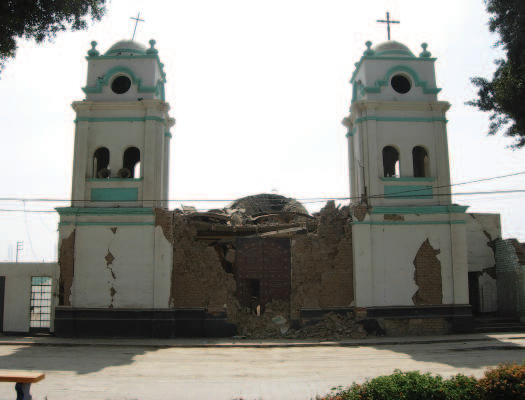
\includegraphics[scale=0.50]{F_Figures/11_Chapter II/Cap2_Imagen3c.png}
	\figurenote{This is a great figure.}
	\label{fig:Figure12}
\end{figure}

Figure~\ref{fig:Figure12} shows this trend. \lipsum[16]

% Capítulo IV: Hipótesis y Variables
% Chapter IV:
\section{Hipótesis y Variables}

% Section 4.1:
\subsection{Hipótesis General}

\lipsum[1]

% Section 4.2:
\subsection{Hipótesis Específicas}

\lipsum[2]

% Section 4.3:
\subsection{Identificación de Variables}

\lipsum[3]

% Section 4.4:
\subsection{Operacionalización de Variables}

\lipsum[4]

% Section 4.5:
\subsection{Matriz de Consistencia}

\lipsum[17]

\lipsum[18]

\begin{figure}[!ht]
  \caption[Cuadro y gráficos que muestran el método N5]{Cuadro y gráficos que muestran el método N5. Adaptado de \cite{deWaal2009}}
  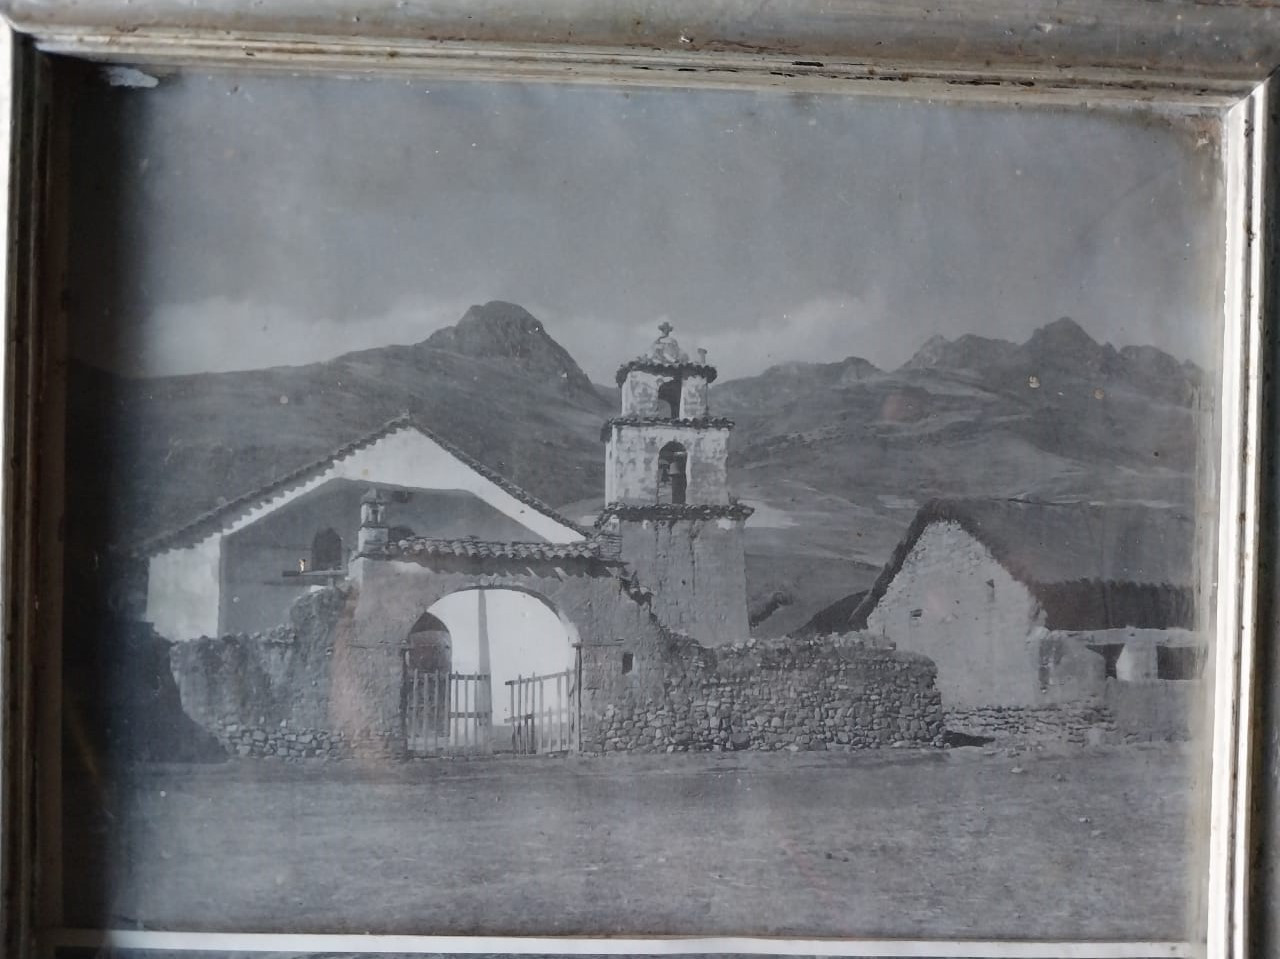
\includegraphics[scale=0.36]{F_Figures/15_Chapter VI/Cap6_Imagen1.jpeg}
  \figurenote{This is a great figure.}
	\label{Cap3_Figura3}
\end{figure}

\lipsum[22] en la Ecuación~\ref{equation124}


\begin{equation}\label{equation124}
  K_{i+1}=K_{i}+\frac{\left ( \delta g_{i}-K_{i}\delta u_{i} \right )c^{T}+c\left ( \delta g_{i}-K_{i}\delta u_{i} \right )^{T}}{c^{T}\delta u_i}-\frac{\left ( \delta g_{i}-K_{i}\delta u_{i} \right )^{T}\delta u_{i} c c^{T}}{\left ( c^{T}\delta u_{i} \right )^{2}}
\end{equation}
\myequations{Ecuación de Emin}

% Capítulo V: Metodología
% Chapter V:
\section{Metodología}

% Section 5.1:
\subsection{Tipo y Diseño de Investigación}

\lipsum[78]

% Section 5.2:
\subsection{Unidad de Análisis}

\lipsum[12]

% Section 5.3:
\subsection{Población de Estudio}

\lipsum[23]

% Section 5.4:
\subsection{Tamaño de Muestra}

\lipsum[25]

% Section 5.5:
\subsection{Selección de Muestra}

\lipsum[22]

% Section 5.6:
\subsection{Técnicas e Instrumentos de Recolección de Datos}

\lipsum[53]

% Section 5.7:
\subsection{Análisis e Interpretación de la Información}

\lipsum[87]

% Capítulo VI: Procedimiento y Método de Análisis
% Chapter VI:
\section{Procedimiento y Método de Análisis}

\subsection{Iglesia Villa de Huayllay}
  
\subsection{Obtención de datos}

\subsection{Implementación MEF}

\subsection{Calibración MEF}

\subsection{Evaluación de la Vulnerabilidad Sísmica sin Refuerzo}

\subsection{Propuesta de Reforzamiento Estructural}

\subsection{Evaluación de la Vulnerabilidad Sísmica con Refuerzo}

% Capítulo VII: Resultados y Discusión
% Chapter VII:
\section{Resultados y Discusión}

\subsection{Resultados}
  
\subsection{Discusión de Resultados}

% Capítulo VIII: Conclusiones y Recomendaciones
% Chapter VIII:
\section{Conclusiones y Recomendaciones}

% Section 8.1:
\subsection{Conclusiones}

\begin{itemize}
    \item \lipsum[1]
    \item \lipsum[2]
    \item \lipsum[3]
    \item \lipsum[4]
    \item \lipsum[5]
\end{itemize}

% Section 8.2:
\subsection{Recomendaciones}

\begin{itemize}
    \item \lipsum[1]
    \item \lipsum[2]
    \item \lipsum[3]
    \item \lipsum[4]
    \item \lipsum[5]
\end{itemize}

\backmatter % Continuar numeración arábica

% Referencias
% Bibliography:
\printbibliography[heading=bibintoc, title={Referencias}]

% Anexos
% Appendix:
\appendix

% Anexo A: Instrument
\section{Instrument}
\label{app:instrument}

As shown in Figure~\ref{fig:Figure2}, these results are impressive. \lipsum[20]

\begin{figure}[ht]
  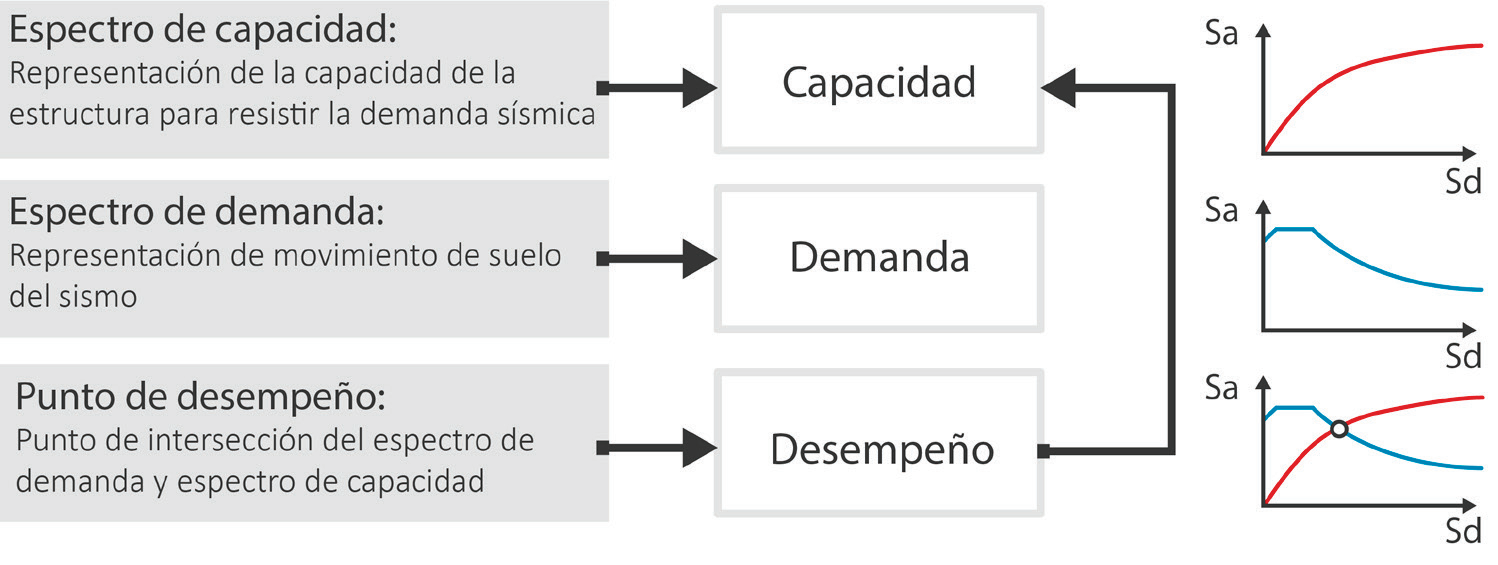
\includegraphics[scale=0.36]{E_IMAGENES/3_Capitulo3/Cap3_Imagen70.png}
	\caption{Cuadro y gráficos que muestran el método N2. Adaptado de \cite{deWaal2009}}
  \figurenote{This is a great figure.}
	\label{fig:Figure2}
\end{figure}

\lipsum[21]
% Pilot Data

\section{Pilot Data}
\label{app:surveydata}

The detailed results are shown in Table~\ref{tab:DeckedTable} from Anexo~\ref{app:surveydata}.

\lipsum[23]

\begin{table}[ht]
  \begin{threeparttable}
    \caption{A More Complex Decked Table}
    \label{tab:DeckedTable}
    \begin{tabular}{@{}lrrr@{}}         \toprule
    Distribution type  & \multicolumn{2}{l}{Percentage of} & Total number   \\
                       & \multicolumn{2}{l}{targets with}  & of trials per  \\
                       & \multicolumn{2}{l}{segment in}    & participant    \\ \cmidrule(r){2-3}
                                    &  Onset  &  Coda            &          \\ \midrule
    Categorical -- onset\tabfnm{a}  &    100  &     0            &  196     \\
    Probabilistic                   &     80  &    20\tabfnm{*}  &  200     \\
    Categorical -- coda\tabfnm{b}   &      0  &   100\tabfnm{*}  &  196     \\ \midrule
    \end{tabular}
    \tablenote{All data are approximate.

            \tabfnt{a}Categorical may be onset.
            \tabfnt{b}Categorical may also be coda.

            \tabfnt{*}\textit{p} < .05.
            \tabfnt{**}\textit{p} < .01.
         }
  \end{threeparttable}
\end{table}

\lipsum[23]

\end{document}

% 
% Derechos de autor (C) 2022 por Diner Sánchez
% 
% Este trabajo se puede distribuir y/o modificar bajo las condiciones de la licencia pública
% GNU GENERAL PUBLIC LICENSE, Version 3, 29 June 2007 o cualquier
% versión posterior.
% 
% Los usuarios pueden modificar estos archivos libremente sin permiso, siempre y cuando
% se mantenga intacta la línea de derechos de autor y esta declaración.
% 
% Este trabajo no cuenta con el respaldo, afiliación o probablemente ni el conocimiento
% de la Universidad San Ignacio de Loyola.
% 
% Este trabajo consiste en el archivo README.md y el archivo de licencia LICENSE.
% Asegúrate de mantener estos archivos al distribuir o modificar el trabajo.
%


